\documentclass[aspectratio=169,11pt]{beamer}

\usepackage[utf8]{inputenc}
\usepackage[T1]{fontenc}
\usepackage[spanish]{babel}
\usepackage{amsmath,amssymb}
\usepackage{tikz}
\usetikzlibrary{arrows.meta,angles}

\usetheme{Madrid}
\usecolortheme{default}
\setbeamertemplate{navigation symbols}{}
\setbeamertemplate{blocks}[rounded][shadow=false]

\newcommand{\ang}[1]{\angle #1^\circ}
\newcommand{\jj}{j}

\title[Números complejos]{Paso 1: Números complejos}
\subtitle{Base para entender la respuesta en frecuencia y QFT}
\author{Curso de control robusto (QFT)}
\date{}

\begin{document}

% ------------------------------------------------------------
\begin{frame}
  \titlepage
\end{frame}

% ------------------------------------------------------------
\begin{frame}{Dónde encaja este paso}
  \tiny
  \begin{enumerate}\setlength{\itemsep}{-2pt}
    \item[\textbf{1.}] \textbf{Números complejos} \hfill $\leftarrow$ estamos aquí
    \item[2.] Funciones de transferencia: $s$, polos y ceros
    \item[3.] Respuesta en frecuencia: $s=j\omega$, magnitud y fase
    \item[4.] Decibelios y escala logarítmica (Bode)
    \item[5.] Realimentación: $L$, $T=\frac{L}{1+L}$, $S=\frac{1}{1+L}$
    \item[6.] Nichols chart
    \item[7.] Incertidumbre y templates
    \item[8.] Especificaciones $\rightarrow$ bounds
    \item[9.] Loop shaping, prefiltro y verificación
    \item[10.] QFT en control digital
    \item[11.] Dos caminos digitales: $z$ y $w$
    \item[12.] Estabilidad, límites, más especificaciones y caso real
    \item[13.] Muestreo por eventos con periodo base $T$
    \item[14.] Sistemas de dos estados: lazo interno y externo
    \item[15.] QFT y sistemas no lineales
    \item[16.] Algoritmos de QFT: cómo funcionan por dentro
    \item[17.] QFT en Python: una biblioteca paso a paso
    \item[18.] QFT en MATLAB: el mismo código, otra sintaxis
    \item[19.] Historia, panorama y bibliografía
  \end{enumerate}
  \vspace{4pt}
  \begin{block}{Objetivo de hoy}
    Poder calcular a mano $P(j\omega)$ y expresarlo como magnitud y fase.
  \end{block}
\end{frame}

% ------------------------------------------------------------
\begin{frame}{Números imaginarios: ¿para qué existen?}
  \begin{block}{El problema}
    \small
    Con los reales, $x^2 = -1$ \textbf{no tiene solución}: ningún real elevado al cuadrado da un número negativo.
    Pero aparece a menudo, p.\,ej. en las raíces de $s^2+2s+5=0$.
  \end{block}

  \uncover<2->{%
  \begin{block}{La solución: inventar el número que falta}
    \small
    Se \emph{define} una unidad nueva $j$ con $j^2=-1$ y se trabaja con números $x+jy$.
    Es ampliar los números, como se inventaron los negativos para poder restar $3-5$.
    Con ellos, \textbf{toda} ecuación polinómica tiene todas sus raíces.
  \end{block}}

  \uncover<3->{%
  \begin{block}{Su razón de ser en ingeniería}
    \small
    \begin{itemize}
      \item \textbf{Giros:} multiplicar por $j$ gira $90^\circ$. Un complejo codifica \emph{tamaño y ángulo}.
      \item \textbf{Senoidales:} $A\cos(\omega t+\varphi)$ se resume en un complejo; derivar es multiplicar por $j\omega$.
      \item \textbf{Control:} polos, ceros y $P(j\omega)$ son complejos; es lo que dibuja QFT.
    \end{itemize}
  \end{block}}
\end{frame}

% ------------------------------------------------------------
\begin{frame}{¿Qué es $j$?}
  \begin{block}{1. Definición}
    $j$ es la \textbf{unidad imaginaria}: el número que cumple $\boxed{j^2 = -1}$ $^{\dagger}$
  \end{block}

  \uncover<2->{%
  \begin{block}{2. Número complejo}
    \small
    Tiene dos partes: $z = x + jy$, con $x$ la \textbf{parte real} e $y$ la \textbf{parte imaginaria}.
    Se suma y se multiplica como un binomio$^{*}$, con la regla $j^2=-1$. Es un \textbf{punto} $(x,y)$ de un plano.
  \end{block}}

  \uncover<3->{%
  \begin{columns}[T]
    \begin{column}{0.48\textwidth}
      \begin{block}{$^{\dagger}$ ¿Por qué $j$ y no $i$?}
        \footnotesize
        En matemáticas se escribe $i$. En electricidad y control, $i$ ya significa \textbf{corriente} ($i(t)$) y ambas aparecerían en las mismas fórmulas. Para no confundirlas se usa $j$. Es el mismo número: $i^2=j^2=-1$.
      \end{block}
    \end{column}
    \begin{column}{0.48\textwidth}
      \begin{block}{$^{*}$ ¿Qué es un binomio?}
        \footnotesize
        Expresión de \textbf{dos términos} unidos por suma o resta, como $x+jy$ o $a+b$. Al multiplicar dos, cada término del primero se multiplica por cada uno del segundo: $(a+b)(c+d)=ac+ad+bc+bd$. Con complejos se aplica después $j^2=-1$.
      \end{block}
    \end{column}
  \end{columns}}
\end{frame}

% ------------------------------------------------------------
\begin{frame}{El plano complejo}
  \begin{columns}[T]
    \begin{column}{0.55\textwidth}
      \centering
      \begin{tikzpicture}[scale=0.62,>=Stealth]
        \draw[->] (-0.5,0) -- (7,0) node[right] {Re};
        \draw[->] (0,-0.5) -- (0,6.5) node[above] {Im};
        \coordinate (O) at (0,0);
        \coordinate (X) at (5,0);
        \coordinate (Z) at (5,5);
        \draw[thick,blue,->] (O) -- (Z) node[midway,above left] {$|z|$};
        \draw[dashed] (Z) -- (X) node[below] {$x=5$};
        \draw[dashed] (Z) -- (0,5) node[left] {$y=5$};
        \fill (Z) circle (2.5pt) node[above right] {$z=5+5j$};
        \pic[draw,->,angle radius=1.1cm] {angle=X--O--Z};
        \node at (1.9,0.7) {$\theta$};
      \end{tikzpicture}
    \end{column}
    \begin{column}{0.45\textwidth}
      \begin{itemize}
        \item Eje horizontal: parte real $x$
        \item Eje vertical: parte imaginaria $y$
        \item La flecha del origen al punto tiene:
        \begin{itemize}
          \item una \textbf{longitud} $|z|$
          \item un \textbf{ángulo} $\theta$
        \end{itemize}
      \end{itemize}
      \vspace{4pt}
      Estas dos medidas dan la \textbf{forma polar}.
    \end{column}
  \end{columns}
\end{frame}

% ------------------------------------------------------------
\begin{frame}{Dos formas de escribir lo mismo}
  \begin{columns}[T]
    \begin{column}{0.48\textwidth}
      \begin{block}{Rectangular}
        \[ z = x + jy \]
      \end{block}
      \begin{block}{Polar}
        \[ z = |z|\angle\theta = |z|\,e^{j\theta} \]
      \end{block}
    \end{column}
    \begin{column}{0.48\textwidth}
      \textbf{De rectangular a polar}
      \[
        |z| = \sqrt{x^2+y^2}, \qquad
        \theta = \operatorname{atan2}(y,x)
      \]
      \textbf{De polar a rectangular}
      \[
        x = |z|\cos\theta, \qquad y = |z|\sin\theta
      \]
    \end{column}
  \end{columns}
  \vspace{6pt}
  \begin{alertblock}{Idea clave}
    Las dos formas describen el mismo punto. Se elige la que haga más fácil la operación.
  \end{alertblock}
\end{frame}

% ------------------------------------------------------------
\begin{frame}{La función $\operatorname{atan2}(y,x)$: definición completa}
  \small
  \[
    \operatorname{atan2}(y,x)=
    \begin{cases}
      \arctan\!\left(\tfrac{y}{x}\right) & x>0\\[3pt]
      \arctan\!\left(\tfrac{y}{x}\right)+180^\circ & x<0,\ y\ge 0\\[3pt]
      \arctan\!\left(\tfrac{y}{x}\right)-180^\circ & x<0,\ y<0\\[3pt]
      +90^\circ & x=0,\ y>0\\[1pt]
      -90^\circ & x=0,\ y<0\\[1pt]
      \text{indefinido} & x=0,\ y=0
    \end{cases}
  \]
  Resultado en $(-180^\circ,\,180^\circ]$. En radianes, $180^\circ=\pi$.

  \begin{alertblock}{¿Por qué no basta $\arctan(y/x)$?}
    El cociente $y/x$ pierde el cuadrante: $1+j$ y $-1-j$ dan ambos $y/x=1$ y $\arctan(1)=45^\circ$.
    Con $\operatorname{atan2}$: $\operatorname{atan2}(1,1)=45^\circ$ y $\operatorname{atan2}(-1,-1)=-135^\circ$.
  \end{alertblock}
\end{frame}

\begin{frame}{$\arctan(y/x)$ frente a $\operatorname{atan2}(y,x)$}
\centering
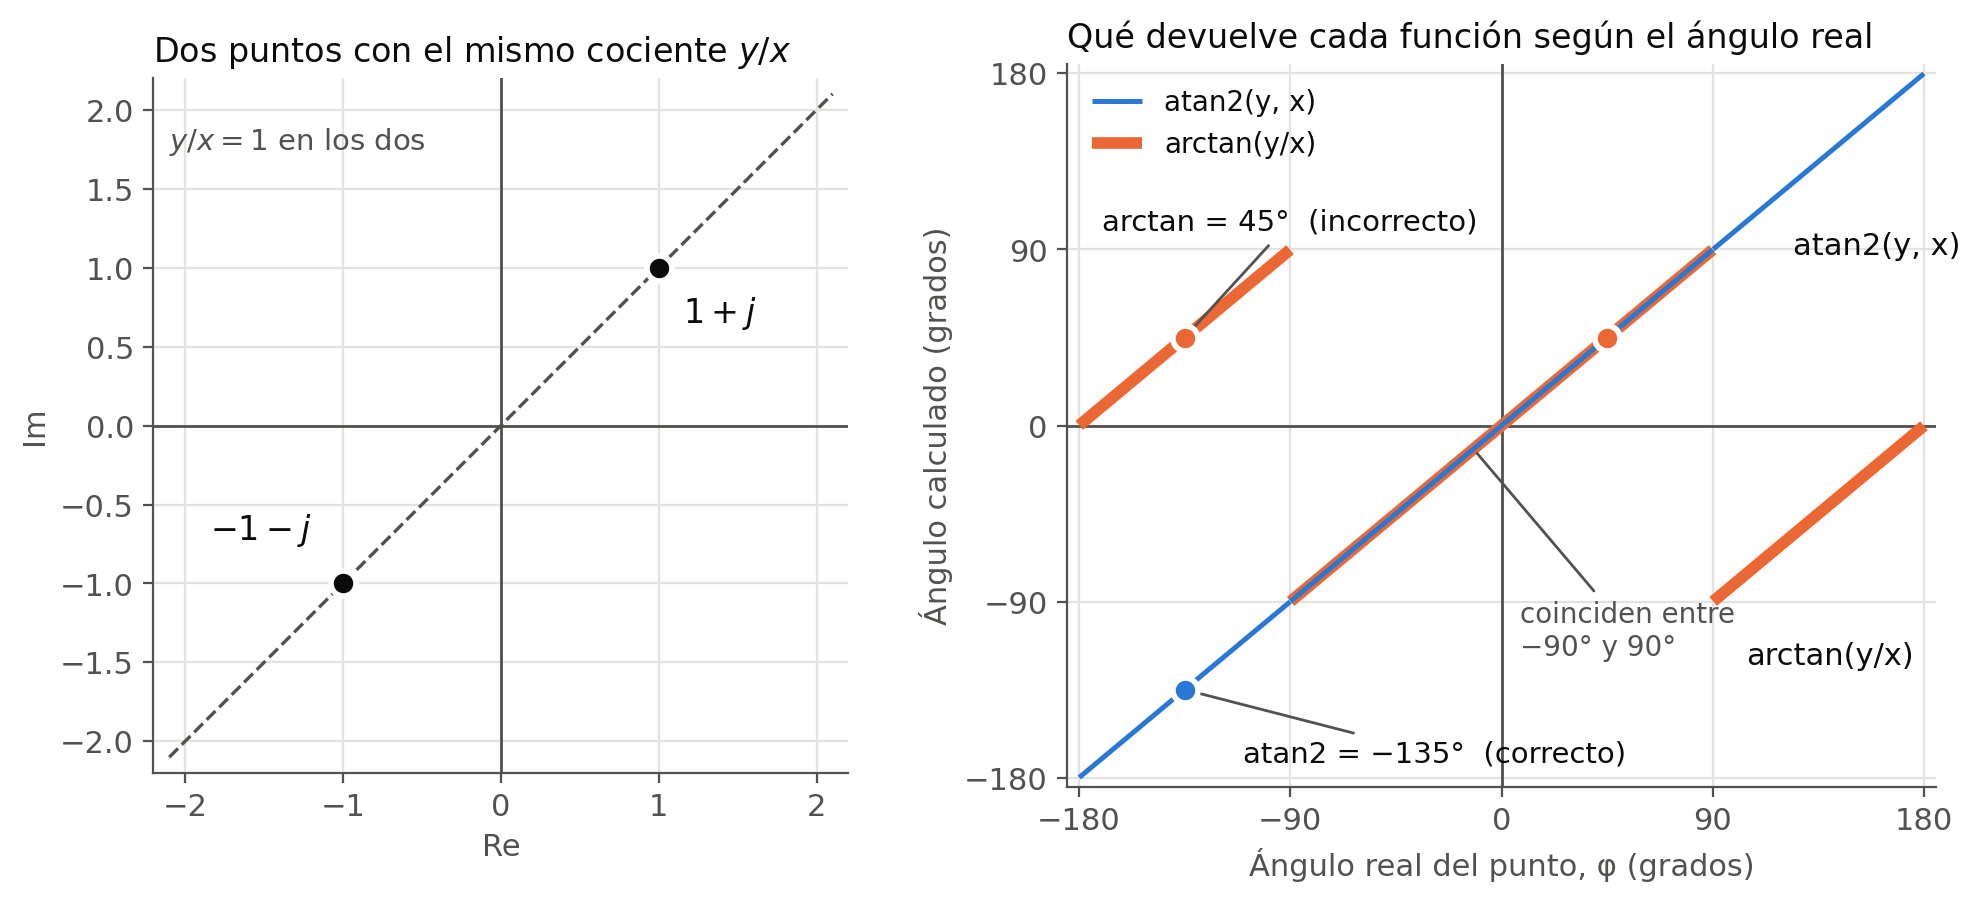
\includegraphics[width=\textwidth,height=0.74\textheight,keepaspectratio]{fig/atan_vs_atan2.png}

\smallskip
\small $1+j$ y $-1-j$ tienen el mismo cociente $y/x$, pero ángulos distintos: solo $\operatorname{atan2}$ usa los signos de $x$ e $y$ para distinguirlos.
\end{frame}


% ------------------------------------------------------------
\begin{frame}{Operaciones}
  \renewcommand{\arraystretch}{1.6}
  \centering
  \begin{tabular}{@{}l p{0.38\textwidth} p{0.38\textwidth}@{}}
    \hline
    & \textbf{Rectangular} & \textbf{Polar} \\
    \hline
    \textbf{Suma} & se suman partes reales e imaginarias por separado & incómoda: conviene pasar a rectangular \\
    \textbf{Producto} & distributiva y $j^2=-1$ & \textbf{magnitudes se multiplican, ángulos se suman} \\
    \textbf{Cociente} & se multiplica por el conjugado & \textbf{magnitudes se dividen, ángulos se restan} \\
    \hline
  \end{tabular}
  \vspace{8pt}

  \begin{block}{Regla que justifica el producto polar}
    \[ e^{j\alpha}\,e^{j\beta} = e^{j(\alpha+\beta)} \]
    Es la misma regla de los exponentes que ya conoces.
  \end{block}
\end{frame}

% ------------------------------------------------------------
\begin{frame}{Suma en polar: por qué hay que pasar por rectangular}
  \small
  \setlength{\parskip}{2pt}
  Con $z_1=3+4j=5\angle 53.13^\circ$ \ y \ $z_2=1+j=1.414\angle 45^\circ$:

  \begin{alertblock}{Error típico: sumar magnitudes y ángulos}
    $5+1.414=6.414$ \ y \ $53.13^\circ+45^\circ=98.13^\circ$ \ $\Rightarrow$ $6.414\angle 98.13^\circ$ \ \textbf{(incorrecto)}\\
    Esa regla es la del \emph{producto} (con ángulos). En la suma no funciona: los vectores se suman \emph{componente a componente}, no longitud con longitud.
  \end{alertblock}

  \begin{block}{Método correcto: 3 pasos}
    \begin{enumerate}
      \item Polar $\to$ rectangular: $x=r\cos\theta$, \ $y=r\sin\theta$. Aquí $5\angle53.13^\circ=3+4j$ y $1.414\angle45^\circ=1+j$.
      \item Sumar por componentes: $(3+1)+(4+1)j=4+5j$.
      \item Rectangular $\to$ polar: $r=\sqrt{4^2+5^2}=6.403$, \ $\theta=\operatorname{atan2}(5,4)=51.34^\circ$.
    \end{enumerate}
    Resultado: $\boxed{6.403\angle 51.34^\circ}$. Como $6.403<6.414$, se ve que la longitud de la suma no es la suma de longitudes.
  \end{block}
\end{frame}

% ------------------------------------------------------------
\begin{frame}{Producto y cociente: la tabla en acción}
  \small
  \setlength{\parskip}{2pt}
  \addtolength{\abovedisplayskip}{-4pt}
  Mismos $z_1=3+4j=5\angle 53.13^\circ$ y $z_2=1+j=1.414\angle 45^\circ$. Calculamos cada operación por \textbf{las dos vías de la tabla}: deben dar lo mismo.

  \begin{block}{Producto \ ($\times$ magnitudes, $+$ ángulos)}
    Rectangular: $(3+4j)(1+j)=3+3j+4j+4j^2=\boxed{-1+7j}$

    Polar: $5\cdot 1.414=7.071$ \ y \ $53.13^\circ+45^\circ=98.13^\circ$ \ $\Rightarrow$ $\boxed{7.071\angle 98.13^\circ}$\\
    Coinciden: $|{-1}+7j|=7.071$ y $\operatorname{atan2}(7,-1)=98.13^\circ$.
  \end{block}
  \begin{block}{Cociente \ ($\div$ magnitudes, $-$ ángulos)}
    Rectangular: $\dfrac{3+4j}{1+j}\cdot\dfrac{1-j}{1-j}=\dfrac{7+j}{2}=\boxed{3.5+0.5j}$

    Polar: $5/1.414=3.536$ \ y \ $53.13^\circ-45^\circ=8.13^\circ$ \ $\Rightarrow$ $\boxed{3.536\angle 8.13^\circ}$
  \end{block}
  \textbf{Para qué sirve:} en QFT $P(j\omega)$ es un cociente de productos de binomios $(j\omega+a)$. En polar es mucho más corto: es lo que haremos en el ejemplo siguiente.
\end{frame}

% ------------------------------------------------------------
\begin{frame}{Ejemplo resuelto (1/3): planteamiento y vía rectangular}
  \small
  \begin{block}{1. El problema}
    Planta nominal: $\displaystyle P(s)=\frac{k}{(s+a)(s+b)}$ con $k=1,\ a=5,\ b=30$. Queremos $P(j\omega)$ en $\omega=5$\,rad/s.
  \end{block}

  \uncover<2->{%
  \begin{block}{2. Sustituir $s=j\omega=5j$}
    $\displaystyle P(j5)=\frac{1}{(5j+5)(5j+30)}=\frac{1}{(5+5j)(30+5j)}$

    El denominador es el \textbf{producto de dos complejos}. Primero lo calculamos.
  \end{block}}

  \uncover<3->{%
  \begin{block}{3. Producto por la vía rectangular (distributiva)}
    \vspace{-4pt}
    \begin{align*}
      (5+5j)(30+5j) &= 5\cdot30 + 5\cdot5j + 5j\cdot30 + 5j\cdot5j\\
                    &= 150 + 25j + 150j + 25j^2 \qquad (j^2=-1)\\
                    &= 150 - 25 + 175j = \boxed{125 + 175j}
    \end{align*}
  \end{block}}
\end{frame}

% ------------------------------------------------------------
\begin{frame}{Ejemplo resuelto (2/3): la misma multiplicación por la vía polar}
  \small
  \setlength{\parskip}{2pt}
  Calculamos otra vez $(5+5j)(30+5j)$, ahora en polar, para ver que sale lo mismo que en (1/3).

  \begin{block}{1. Pasar cada factor a polar \ ($r=\sqrt{x^2+y^2}$, \ $\theta=\operatorname{atan2}(y,x)$)}
    $5+5j=\sqrt{50}\,\angle\arctan\tfrac55=7.071\,\ang{45}$\\
    $30+5j=\sqrt{925}\,\angle\arctan\tfrac{5}{30}=30.414\,\ang{9.46}$
  \end{block}

  \uncover<2->{%
  \begin{block}{2. Multiplicar magnitudes y sumar ángulos}
    $7.071\cdot30.414=215.05$ \qquad $45^\circ+9.46^\circ=54.46^\circ$\\
    $\Rightarrow\ (5+5j)(30+5j)=\boxed{215.05\,\ang{54.46}}$
  \end{block}}

  \uncover<3->{%
  \begin{block}{3. Comprobación: ¿coincide con el resultado de (1/3)?}
    En (1/3) obtuvimos $125+175j$. Lo pasamos a polar con las mismas fórmulas:\\
    $r=\sqrt{125^2+175^2}=\sqrt{46250}=215.05$ \quad $\theta=\operatorname{atan2}(175,125)=54.46^\circ$\\
    (como $x=125>0$, vale $\arctan(175/125)$). \textbf{Coincide}: las dos vías dan el mismo número.
  \end{block}}
\end{frame}

% ------------------------------------------------------------
\begin{frame}{Ejemplo resuelto (3/3): el resultado $P(j5)$}
  \[
    P(j5)=\frac{1}{215.05\,\ang{54.46}}
    = 0.00465\,\ang{-54.46}
  \]
  \begin{itemize}
    \item Dividir por un complejo: se \textbf{dividen} magnitudes y se \textbf{resta} el ángulo.
    \item Por eso el denominador aporta \textbf{fase negativa}.
  \end{itemize}
  \vspace{4pt}
  En decibelios:
  \[
    20\log_{10}(0.00465) = \boxed{-46.65\ \text{dB}}
  \]
  \centering
  \textbf{Magnitud: $-46.65$ dB \qquad Fase: $-54.46^\circ$}

  \vspace{6pt}
  \begin{block}{;) Nota}
    \footnotesize
    ¿Para qué sirven los decibelios? Más adelante lo verás: es lo que convierte los productos en sumas y hace posible el loop shaping. Por ahora, basta saber que $\log_{10}(x)=y$ significa $10^y=x$.
  \end{block}
\end{frame}

% ------------------------------------------------------------
\begin{frame}{¿Cómo se calcula el logaritmo?}
  \small
  \setlength{\parskip}{2pt}
  \begin{block}{Definición}
    $\log_{10}(x)$ es el \textbf{exponente} al que hay que elevar 10 para obtener $x$: \ $\log_{10}(x)=y \iff 10^y=x$.\\
    $\log_{10}(100)=2$ \ porque $10^2=100$. \qquad $\log_{10}(0.001)=-3$ \ porque $10^{-3}=0.001$.
  \end{block}

  \uncover<2->{%
  \begin{block}{Con números que no son potencias de 10: separar la potencia}
    $0.00465 = 4.65\cdot10^{-3}$, y el log de un producto es la suma de logs:\\
    $\log_{10}(0.00465)=\log_{10}(4.65)+\log_{10}(10^{-3})=0.6675-3=-2.3325$\\
    Ahora el factor 20 de los decibelios: \ $20\cdot(-2.3325)=\boxed{-46.65\ \text{dB}}$
  \end{block}}

  \uncover<3->{%
  \begin{block}{¿Y $\log_{10}(4.65)=0.6675$?}
    No se hace a mano: sale de la calculadora o de Python (\texttt{math.log10(4.65)}). A mano solo es fácil para potencias de 10.
    \textbf{Referencias útiles} (magnitudes, $20\log_{10}$): \ $\times10\to20$\,dB, \ $\times2\to6$\,dB, \ $\times1\to0$\,dB.
  \end{block}}
\end{frame}

% ------------------------------------------------------------
\begin{frame}{El logaritmo en una gráfica}
  \centering
  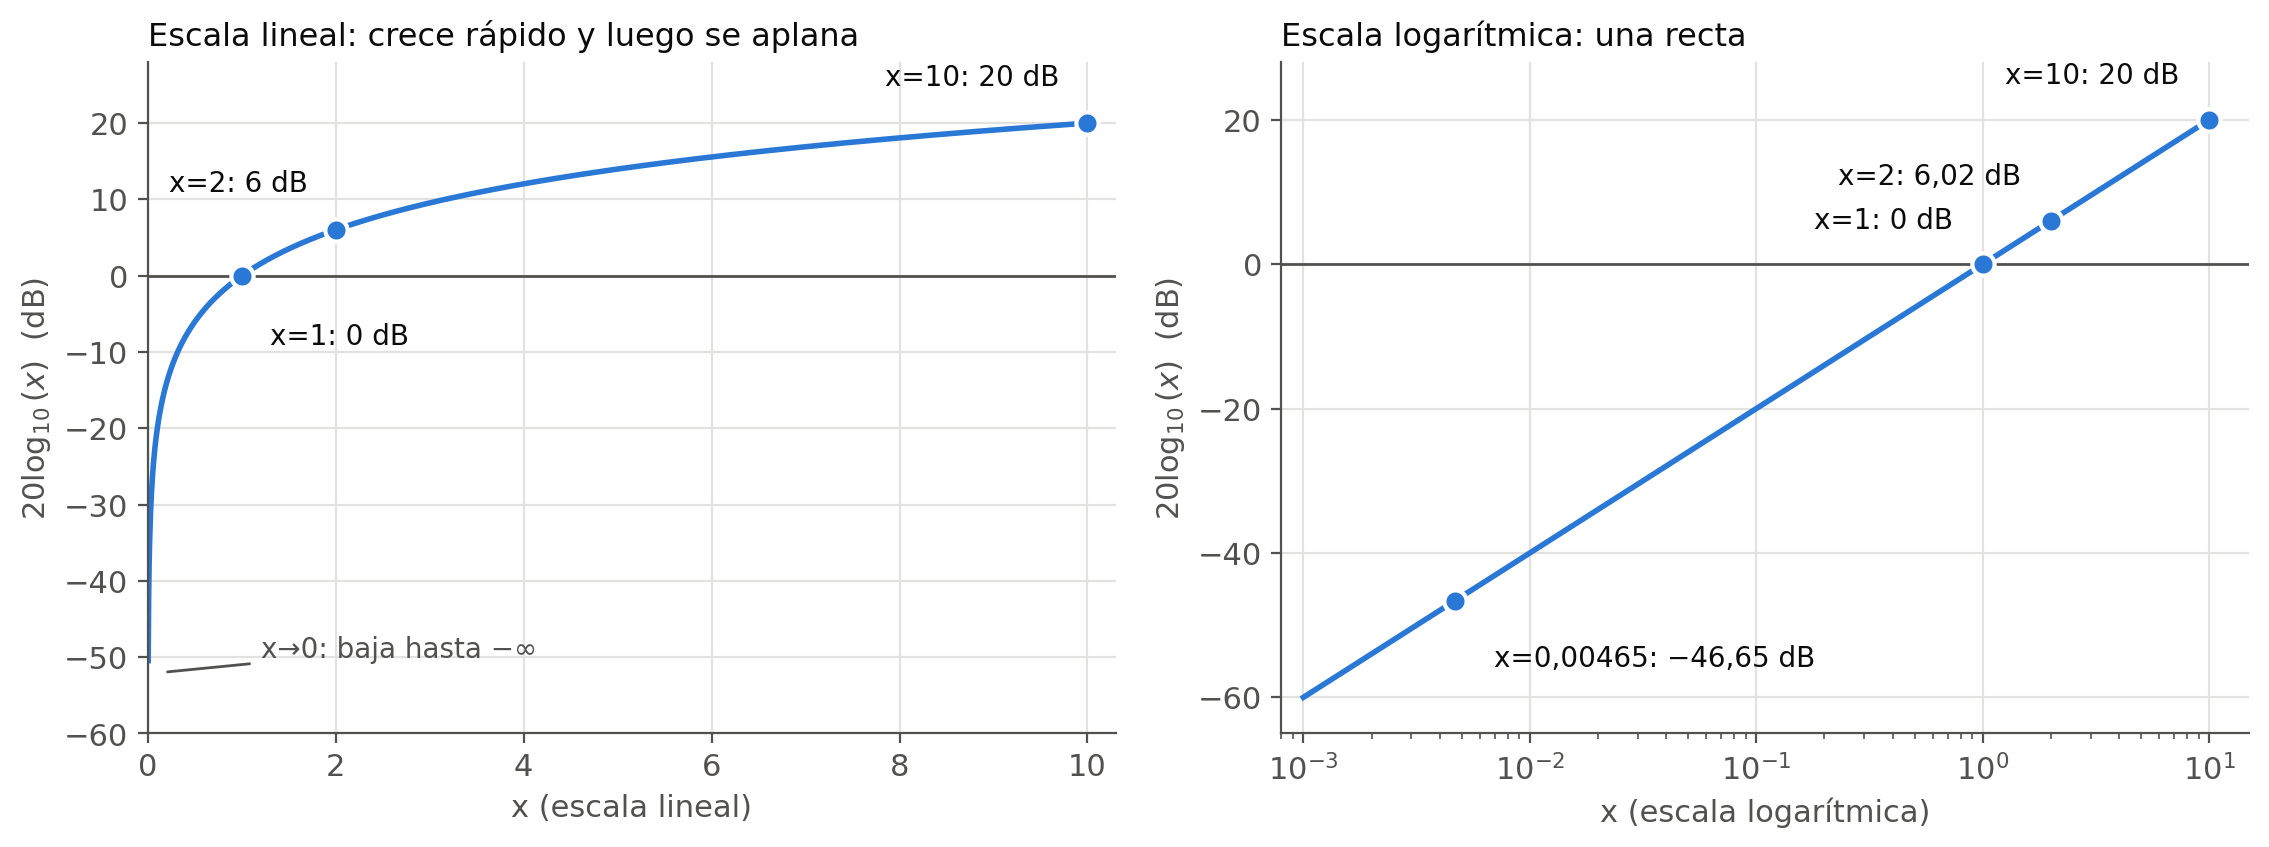
\includegraphics[width=\textwidth,height=0.72\textheight,keepaspectratio]{fig/log_db.png}

  \smallskip
  \small En escala logarítmica, multiplicar por 10 siempre suma 20\,dB: la curva se convierte en una \textbf{recta}. Por eso los decibelios convierten productos en sumas.
\end{frame}

% ------------------------------------------------------------
\begin{frame}{Por qué importa: el ejemplo, visto como sumas}
  \small
  \setlength{\parskip}{2pt}
  Volvemos al ejemplo resuelto: $P(j5)=\dfrac{1}{(5+5j)(30+5j)}$. Cada factor del denominador aporta su propia magnitud y su propio ángulo:

  \begin{center}
    \renewcommand{\arraystretch}{1.1}
    \begin{tabular}{lrr}
      \hline
      & \textbf{Magnitud (dB)} & \textbf{Fase} \\
      \hline
      $1/(5+5j)$ & $-16.99$ & $-45^\circ$ \\
      $1/(30+5j)$ & $-29.66$ & $-9.46^\circ$ \\
      \hline
      \textbf{Total} $P(j5)$ & $\boxed{-46.65}$ & $\boxed{-54.46^\circ}$ \\
      \hline
    \end{tabular}
  \end{center}

  \uncover<2->{%
  \begin{alertblock}{La idea clave}
    En dB y en grados, \textbf{multiplicar factores es sumar sus contribuciones}. No hace falta multiplicar complejos: se suman filas de una tabla.
  \end{alertblock}}

  \uncover<3->{%
  \begin{block}{Y esto, ¿para qué en QFT?}
    Más adelante veremos que el controlador se diseña añadiendo factores (polos y ceros) al sistema, y cada uno \textbf{suma} una curva conocida de dB y grados. Por eso el diseño a mano es viable. (Pasos 5 a 9.)
  \end{block}}
\end{frame}

% ------------------------------------------------------------
\begin{frame}{Ejercicio}
  Calcula $P(j10)$ para $k=1,\ a=5,\ b=30$:
  \begin{enumerate}
    \item Escribe los dos factores del denominador: $j\omega+a$ y $j\omega+b$ con $\omega=10$.
    \item Pásalos a forma polar (magnitud y ángulo de cada uno).
    \item Multiplícalos en polar y calcula $P(j10)=\dfrac{1}{\,\cdots\,}$.
    \item Da el resultado en \textbf{dB} y en \textbf{grados}.
    \item Compruébalo multiplicando en forma rectangular.
  \end{enumerate}
  \vspace{4pt}
  \begin{block}{Para pensar}
    ¿La magnitud sube o baja al pasar de $\omega=5$ a $\omega=10$? ¿Y la fase?
  \end{block}
\end{frame}

% ------------------------------------------------------------
\begin{frame}{Para programarlo: el notebook de este paso}
  \small
  Todo lo de este paso se puede \textbf{ejecutar} en el notebook \texttt{notebooks/paso01\_numeros\_complejos.ipynb}.
  \begin{itemize}
    \item Python: \texttt{1j}, \texttt{abs}, \texttt{np.angle}, \texttt{np.arctan2}, funciones propias y pruebas con \texttt{assert}; la tabla de $P(j\omega)$ en una línea.
    \item Cada cálculo a mano de las diapositivas se \textbf{comprueba} en código.
    \item Incluye celdas \emph{Tu turno} con el ejercicio del paso y la solución plegada.
  \end{itemize}
  \footnotesize Requisitos: \texttt{numpy}, \texttt{matplotlib} y, en el paso 2, \texttt{scipy}.
\end{frame}

\begin{frame}{Resumen}
  \begin{itemize}
    \item $j^2=-1$; un complejo $x+jy$ es un punto del plano.
    \item Forma rectangular para \textbf{sumar}; forma polar para \textbf{multiplicar y dividir}.
    \item Producto: magnitudes $\times$, ángulos $+$. Cociente: magnitudes $\div$, ángulos $-$.
    \item $i$ (matemáticas) y $j$ (ingeniería) son el mismo número.
    \item En dB, los productos de magnitudes son sumas: la base del loop shaping.
  \end{itemize}
  \vspace{6pt}
  \begin{block}{Siguiente paso}
    Paso 2: funciones de transferencia, polos y ceros.
  \end{block}
\end{frame}

\appendix
% ------------------------------------------------------------
\begin{frame}
  \centering
  \vspace{1.2cm}
  {\Huge\bfseries Apéndice}
\end{frame}

% ------------------------------------------------------------
\begin{frame}{Equivalencia con las matemáticas que usan $i$}
  \textbf{$i$ y $j$ son exactamente el mismo número}: $i^2=j^2=-1$.
  \vspace{4pt}

  En electricidad y control $i$ ya significa \emph{corriente}, así que se usa $j$.
  \vspace{6pt}

  \centering
  \renewcommand{\arraystretch}{1.5}
  \begin{tabular}{ll}
    \hline
    \textbf{Matemáticas} & \textbf{Ingeniería} \\
    \hline
    $z = x + iy$ & $z = x + jy$ \\
    $e^{i\theta} = \cos\theta + i\sin\theta$ & $e^{j\theta} = \cos\theta + j\sin\theta$ \\
    $\bar z = x - iy$ & $z^{*} = x - jy$ \\
    $\arg z$ & fase \\
    \hline
  \end{tabular}
  \vspace{6pt}

  \raggedright
  Basta sustituir $i \to j$. La forma $|z|\angle\theta$ es abreviatura de $|z|e^{j\theta}$.
\end{frame}


% ------------------------------------------------------------
\begin{frame}{Dos trampas habituales}
  \begin{block}{En programación}
    \begin{itemize}
      \item Python escribe \texttt{1j} (con el número delante): \texttt{3+4j}. Una \texttt{j} sola es una variable.
      \item MATLAB acepta \texttt{i} y \texttt{j}, pero se pisan si los usas como variable de bucle.
    \end{itemize}
  \end{block}
  \begin{alertblock}{Convención de signo}
    Algunos textos de física usan $e^{-i\omega t}$ y los de ingeniería $e^{+j\omega t}$. Con la de física, la fase sale con \textbf{signo contrario}.

    En control y en QFT se usa la de ingeniería: un retardo es \textbf{fase negativa}.
  \end{alertblock}
\end{frame}


% ------------------------------------------------------------
\begin{frame}{Para curiosos: suma en polar directa (ley de cosenos)}
  \small
  \setlength{\parskip}{2pt}
  Sí se puede: dos vectores y su suma forman un triángulo, y se aplica la \textbf{ley de cosenos}. Con $z_1=r_1\angle\theta_1$ y $z_2=r_2\angle\theta_2$, sea $\Delta=\theta_2-\theta_1$:
  \[
    |z_1+z_2|=\sqrt{r_1^2+r_2^2+2r_1r_2\cos\Delta},
    \qquad
    \angle(z_1+z_2)=\theta_1+\operatorname{atan2}\!\big(r_2\sin\Delta,\; r_1+r_2\cos\Delta\big)
  \]
  \begin{block}{Con nuestro ejemplo: $5\angle53.13^\circ$ y $1.414\angle45^\circ$, \ $\Delta=-8.13^\circ$}
    $|z_1+z_2|=\sqrt{25+2+2\cdot5\cdot1.414\cos(-8.13^\circ)}=\sqrt{41.0}=6.403$\\
    $\angle=53.13^\circ+\operatorname{atan2}(1.414\sin(-8.13^\circ),\;5+1.414\cos(-8.13^\circ))=53.13^\circ-1.79^\circ=51.34^\circ$
  \end{block}
  Mismo resultado que por rectangular: $6.403\angle51.34^\circ$.

  \begin{alertblock}{Pero no ahorra trabajo}
    Sigue necesitando $\sin$ y $\cos$, y la fórmula es más larga que pasar a rectangular, sumar y volver. Por eso en la práctica se convierte: la suma se hace en rectangular y el producto y el cociente en polar.
  \end{alertblock}
\end{frame}



% ------------------------------------------------------------
\begin{frame}{Solución del ejercicio: $P(j10)$ con $k=1,\ a=5,\ b=30$}
  \footnotesize
  \setlength{\parskip}{1pt}
  \begin{block}{1--2. Factores del denominador (rectangular y polar)}
    $5+10j=11.180\,\ang{63.43}$ \qquad $30+10j=31.623\,\ang{18.43}$
  \end{block}
  \begin{block}{3--4. Producto en polar, $P(j10)$, dB y grados}
    $11.180\cdot31.623=353.55$ \quad $63.43^\circ+18.43^\circ=81.87^\circ$ \quad $\Rightarrow$ \quad $P(j10)=\dfrac{1}{353.55\,\ang{81.87}}=0.002828\,\ang{-81.87}$\\
    $20\log_{10}(0.002828)=\boxed{-50.97\ \text{dB}}$ \qquad Fase: $\boxed{-81.87^\circ}$
  \end{block}
  \begin{block}{5. Comprobación en rectangular}
    $(5+10j)(30+10j)=150+50j+300j+100j^2=50+350j$, \ $|50+350j|=353.55$, \ $\operatorname{atan2}(350,50)=81.87^\circ$ \ \textbf{Coincide.}
  \end{block}
  \begin{alertblock}{Para pensar}
    De $\omega=5$ a $\omega=10$ la magnitud \textbf{baja} ($-46.65\to-50.97$\,dB) y la fase es \textbf{más negativa} ($-54.46^\circ\to-81.87^\circ$).
  \end{alertblock}
\end{frame}

\end{document}
